\subsection{NP-completeness}
A problem $B$ is NP-complete if 
\begin{itemize}
	\item $B \in \text{NP}$
	\item For any $A \in \text{NP}, A \preccurlyeq_P B$.  
\end{itemize}

So if $B$ is NP-complete and we solve $B$ in polynomial time, we would solve all problems in NP in polynomial time.

NP-complete problems are the hardest problem in NP. Note that there are even harder problems that lie outside of NP. NP-hard problems are a superset of NP-complete problems.

If we can show just the second property above for a problem $B$, $B$ is said to be NP-hard.

\subsection{Proving NP-Completeness}
Proving that problem $B$ is NP-complete seems difficult, we need to show a polynomial time reduction from every problem in NP to B. But there are infinitely many problems in NP!

Moreover, proving that the first problem in NP-complete is challenging, but luckily, it's been done for us with the help of the Cook-Levin theorem. Cook-Levin theorem proves that circuit-satisfiability is NP-complete.

\subsubsection{Transitivity of Reductions}
Once we have Cook-Levin theorem proof, it is not as difficult to prove other problems NP-complete. Suppose we already know that problem $A$ is NP-complete. This means that $A \in \text{NP}$ and all problem in NP reduce to $A$. Now suppose we want to prove that problem $B$ is NP-complete. We have to show that $B \in \text{NP}$, which is usually not hard. We then have to reduce all problem in NP to B.

Suppose instead, we just reduce $A$ to $B$.For any problem $C \in \text{NP}$, we already know $C$ reduces to $A$ (since $A$ is NP-complete). So $C$ reduces to $A$, which reduces to $B$.

If we can show that polynomial time reduction are \textbf{transitive}, which means if $C$ reduces to $A$ and $A$ reduces to $B$ then $C$ reduces to $B$. Then we would have shown that all problems in NP reduce to $B$.

\begin{figure}[H]
	\centering
	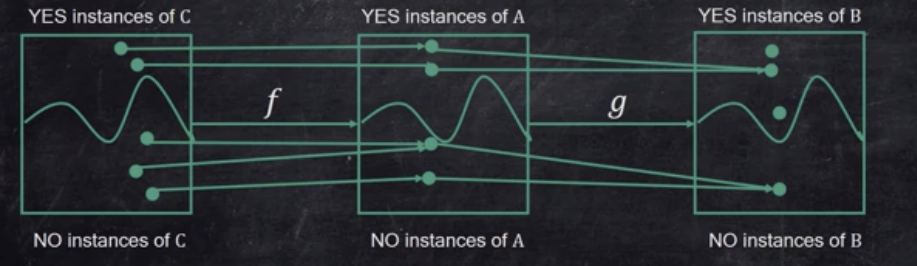
\includegraphics[width=0.5\textwidth]{fig/transitivity-reduction.png}
\end{figure}

In the example, each square represents all possible inputs to that problem and there is infinity many of them. There are some arbitrary unknown partitional inputs into those that are YES instances and those that are No instances. For examples, we draw those arbitrary curves within each of the rectangles. The points above are suppose to be the YES instances of the problem and the points below are the NO instances of the problem. 

Remember that reduction perverse the answer. So the fact that C is reduced to A means that some function $f$ which maps every point in the domain of C to the second box, which is instances of problem A while preserving the answer. Moreover, we just done reduction from A to B by function $g$, which is also answer-preserving.

Then let $x$ be any instance of $C$. $g(f(x))$ is an instance of $B$. Furthermore, $x$ is a YES instance if and only if $g(f(x))$ is a YES instance. So $g(f(x))$ looks like a reduction from $C$ to $B$. The composed function is actually poly-time because of the compositional properties of polynomials.

\subsection{Recipe For Proving a Problem NP-Complete}
To show problem $B$ is NP-complete,
\begin{itemize}
	\item First show $B \in \text{NP}$.
	\item Take a known NP-complete problem A.
	\item Construct a poly-time reduction from A to B.
	\item Prove that the reduction is poly-time and correct, i.e. maps YES instances of A to YES instances of B and NO instances of A to NO instances of B.
\end{itemize}

By transitivity of reductions, since we know all problems in NP reduce to A, we will have shown that all problems in NP reduce to B. So $B$ is NP-complete.










